\section{Problems with the Rarita-Schwinger field}
\begin{frame}
	\frametitle{Coupling the Rarita-Schwinger field to the Photon field}
	We use the general description of gauge-invariance get the coupled Lagrangian $i\partial_\mu\rightarrow D_\mu=i\partial_\mu+eA_\mu$:
	\begin{equation*}
		\symcal{L}_{EM} = \frac{1}{2}\overline\Psi_\nu\l(-\epsilon^{\nu\mu\kappa\lambda}\gamma_5\gamma_\mu\l(\partial_\kappa-ieA_\kappa\r)+\frac{1}{2}m[\gamma^\nu, \gamma^\lambda]\r)\Psi_\lambda	
	\end{equation*}
	\pause
	\begin{align*}
		\frac{\delta \symcal{L}}{\delta \overline\Psi_\nu}=0=
		\l(-\epsilon^{\nu\mu\kappa\lambda}\gamma_5\gamma_\mu\l(\partial_\kappa-ieA_\kappa\r)+\frac{1}{2}m[\gamma^\nu, \gamma^\lambda]\r)\Psi_\lambda
		= T^\nu                                                                                                                                                                      \\
		\overset{\partial_\nu T^\nu}{\Rightarrow}
		[\slashed{\partial},\gamma^\lambda]\Psi_\gamma= 2ie\epsilon^{\nu\mu\kappa\lambda}\gamma_5\gamma_\mu\partial_\nu A_\kappa\Psi_\lambda \qquad
		\dots\Rightarrow \gamma_\mu \Psi^\mu = \frac{2e}{3m^2}\gamma_\mu \widetilde F^{\mu\nu}\Psi_\nu
	\end{align*}
	With $\widetilde F^{\mu\nu}=\frac{1}{2}\epsilon^{\alpha\beta\mu\nu}F_{\alpha\beta}$ and $F^{\mu\nu}=\partial^\mu A^\nu-\partial^\nu A^\mu$.
	
\end{frame}
\begin{frame}
	\frametitle{The Velo-Zwanziger Problem}
	With this coupling Velo and Zwanziger \footnote{\fullcite{velo1969propagation}} showed, that in reference frames with 
	\begin{equation*}
		\abs{\vec B} = \l(\frac{3m^2}{2e}\r)^2
	\end{equation*}
	some of the field components propagate faster than light.
	\vspace{-1em}
	\pause
	\begin{figure}
	\begin{center}
	\begin{tikzpicture}[scale=0.8, transform shape]
		\node at (0, 0) {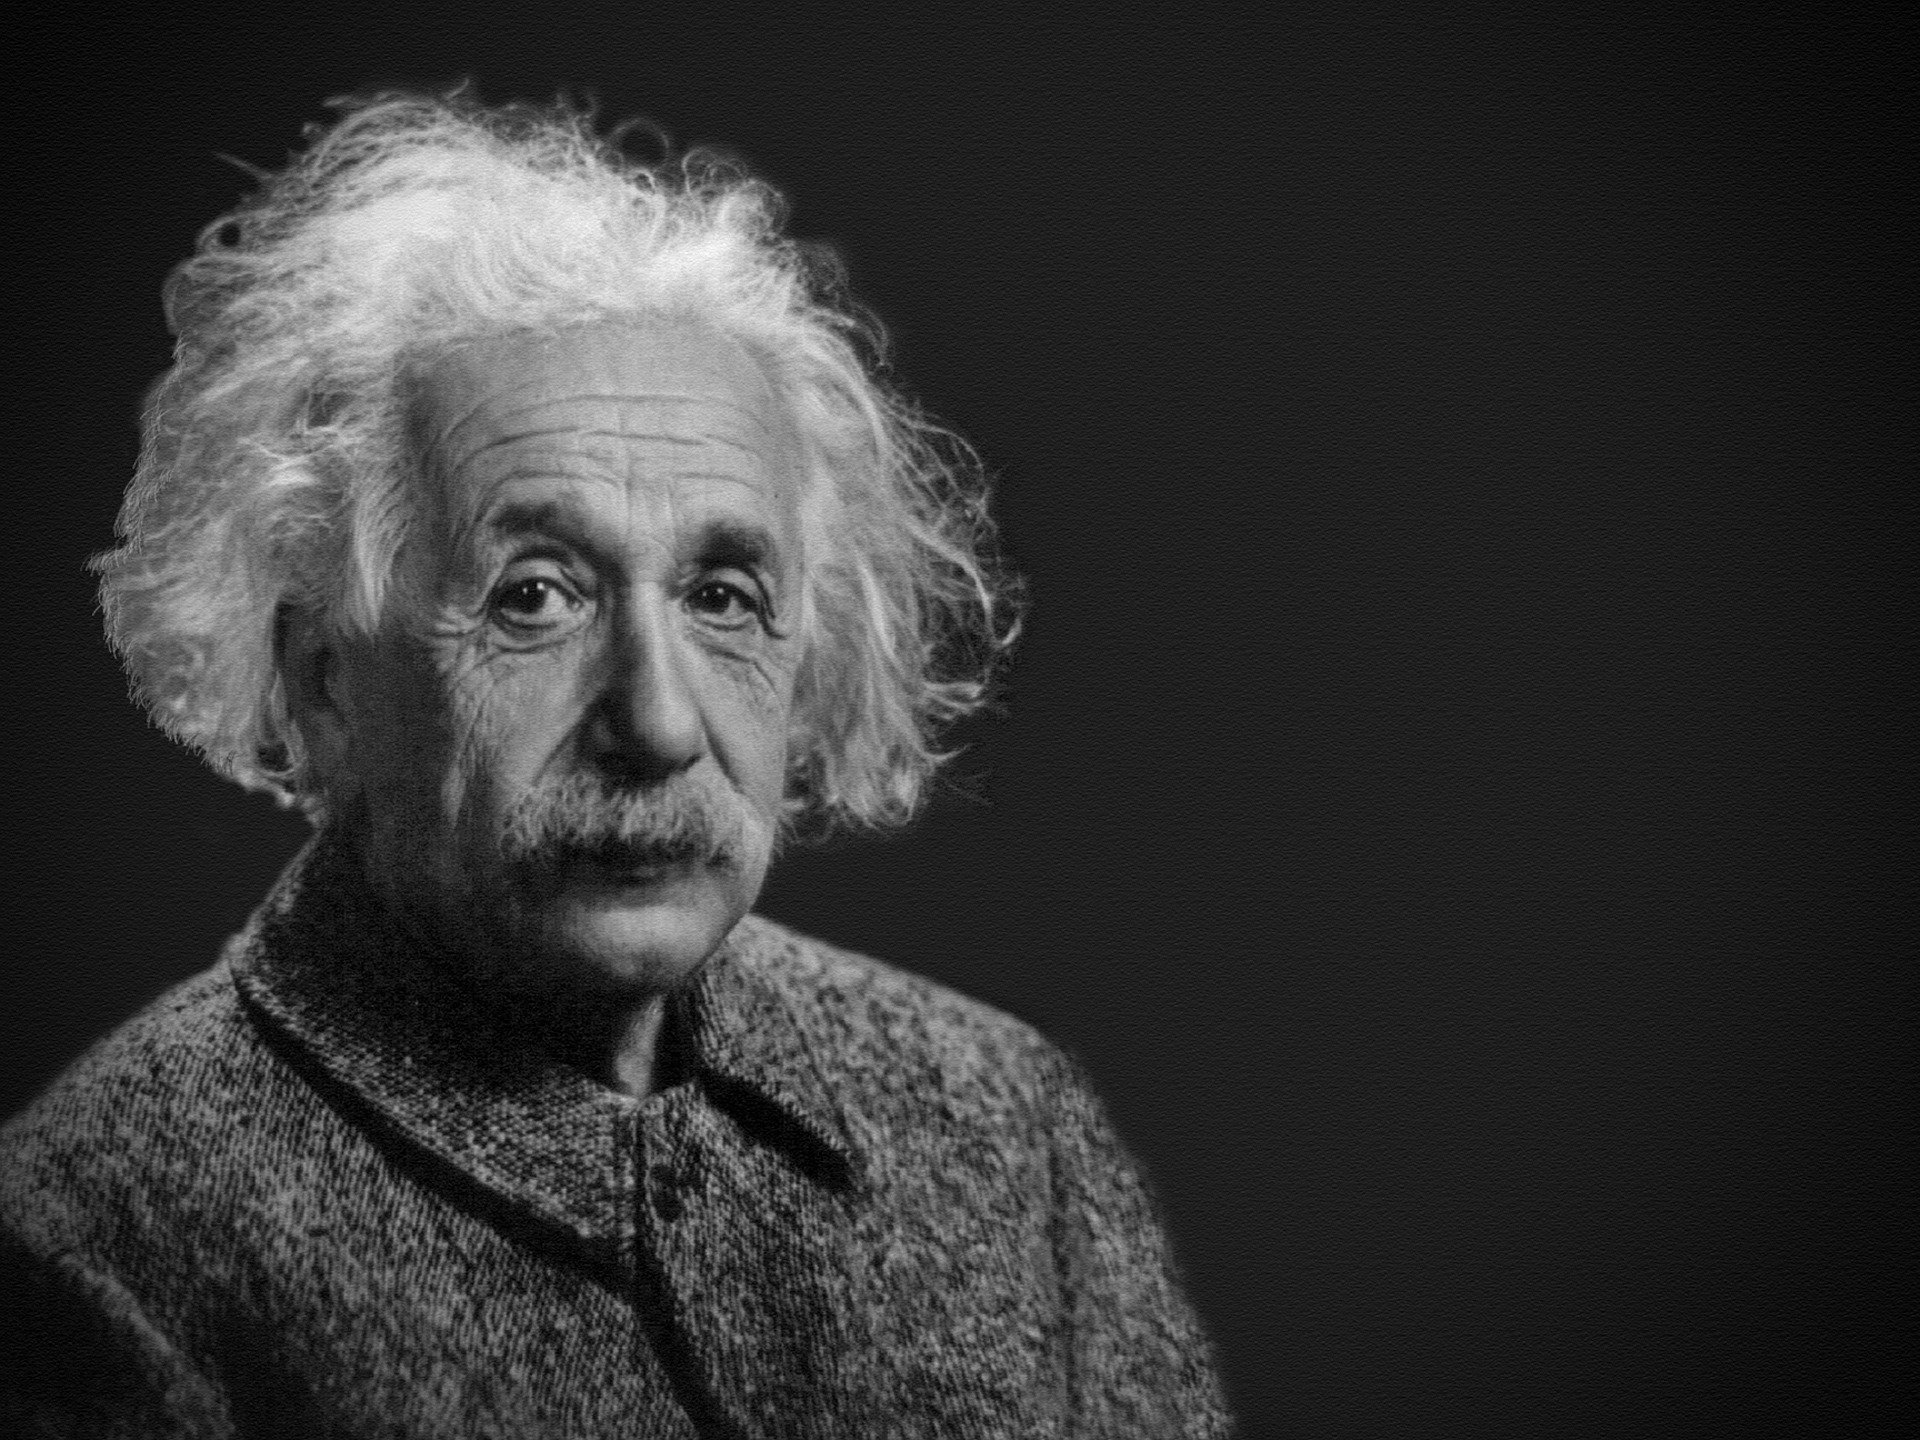
\includegraphics[trim=0 0 500 0, clip, width=0.2\textwidth]{media/einstein.jpg} };
		\node at (0.8, 0) {\Huge\alert{?}};
	\end{tikzpicture}
	\end{center}
	\label{fig:}
	\end{figure}
	\vspace{-1em}
	This is caused by not having enough contraints anymore. For the same reason Johnson and
	Sudarshan found inconsistencies in quantization of the RS-Field in presence of EM couplling 8 years earlier
	\footnote{\fullcite{PILLING_2005}}.
	\vspace{1em}
\end{frame}
\begin{frame}
	\frametitle{Weinbergs view on problems with the RS-Field}
	In \fullcite[243]{weinberg1995quantum} Weinberg 
	doubts the physical relevance of these problems: 
	\begin{enumerate}
		\item No problems in pertubation theory description of RS-Coupling 
		\item In more complicated interactions no one has shown that the problems persist
		\item Existing $\sfrac{3}{2}$ fermions are not point-like and thus have a more complicated interaction
		\item Problems may also be solved by switching the representation 
		\item \emph{Kaluza-Klein}, \emph{Stringtheory} and \emph{Supergravity} all consistently quantize interacting $s\geq\sfrac{3}{2}$ fermions
	\end{enumerate}
	
\end{frame}
